\documentclass[a4paper, 10pt, final, garamond]{book}
\usepackage{cours-preambule}
\graphicspath{{./figures/}}

\makeatletter
\renewcommand{\@chapapp}{Contr\^ole de connaissances}
\makeatother

\toggletrue{student}
\HideSolutionstrue

\begin{document}
\setcounter{chapter}{3}

\chapter{Électrocinétique~: condensateurs et bobines}

\ifstudent{
	\begin{tikzpicture}[remember picture, overlay]
		\node[anchor=north west, align=left]
		at ([shift={(1.4cm,0)}]current page.north west)
		{\\[5pt]\Large\bfseries Nom~:\\[10pt]\Large\bfseries Prénom~:};
		\node[anchor=north east, align=right]
		at ([shift={(-1.5cm,-17pt)}]current page.north east)
		{\Large\bfseries Note~:\hspace{1cm}/10};
	\end{tikzpicture}
}

\begin{enumerate}[label=\sqenumi, leftmargin=10pt]
	\nitem{5}
	\noindent
	\begin{minipage}[t]{.69\linewidth}
    On suppose le circuit RC série suivant, en échelon de tension montant. On
    suppose le condensateur initialement déchargé, et on ferme l'interupteur à
    $t=0$. Déterminer l'équation différentielle sous forme canonique de $u_C$
    pour $t \geq 0$, donner la condition initiale et comment la déterminer, et
    résoudre l'équation différentielle.
	\end{minipage}
	\hfill
	\begin{minipage}[t]{.29\linewidth}
		~
		\vspace{-30pt}
		\begin{center}
			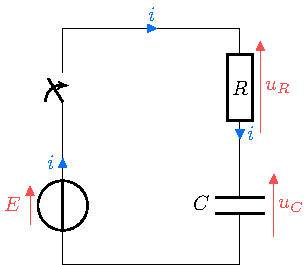
\includegraphics[width=.9\linewidth]{circ_rc-start}
			\captionof{figure}{}
		\end{center}
	\end{minipage}
	\begin{isd}
		\wsw{
		Avec la loi des mailles,
		\begin{DispWithArrows*}
			u_R + u_C &= E
			\Arrow{$u_R = Ri$\\et $i = C \dv{u_C}{t}$}
			\\\Lra
			RC \dv{u_C}{t} + u_C        & = E
			\Arrow{$\tau = RC$}
			\\\Lra
			\dv{u_C}{t} + \frac{1}{\tau}u_C & = \frac{E}{\tau}
		\end{DispWithArrows*}
		L'équation homogène est~:
		\[
			\dv{u_{C,h}}{t} + \frac{1}{\tau}u_{C,h} = 0
		\]
		La forme générale de la solution pour cette équation est~:
		\[
			u_{C,h}(t) = A\exp\left( -\frac{t}{\tau} \right)
		\]
		}
		\tcblower
		\wsw{
			Une solution particulière avec $u_{C,p}(t) = \lambda$ donne
			\[
				0 + \frac{\lambda}{\tau} = \frac{E}{\tau}
			\]
			Donc $u_{C,p}(t) = E$ est \textbf{une} solution de l'équation
			différentielle.
			La solution générale est donc
			\[
				u_C(t) = E + A\exp \left( - \frac{t}{\tau} \right)
			\]
			La condition initiale est, par continuité de $u_C(t)$,
			\[
				u_C(t=0) = 0
				\qqet
				u_C(0) = A + E \Ra A=-E
			\]
			Ainsi,
			\[
				\boxed{u_C(t) = E\left(1-\exp\left(-\frac{t}{\tau}\right)\right)}
			\]
		}
	\end{isd}
  \nitem{5} Démontrer, à l'aide d'un schéma, l'association

\end{enumerate}
\end{document}
